\documentclass{ximera}
\title{Continuity and Discontinuity}
\begin{abstract}
\end{abstract}
\begin{document}
\maketitle
\begin{dialogue}
\item[Julia]What does it mean for a graph to be discontinuous? I don't get it!
\item[Dylan] I think it's like when there's a hole in the graph or something.
\item[James] Actually there are different kinds of discontinuities, but it's hard to visualize so let's take a look!
\item[Altogether] LET'S DIVE IN!
\end{dialogue}
\section{Introduction}
\begin{question}
A function $f$ is said to be \textit{continuous at a point} $x = a$ if which three conditions are satisfied?
\begin{selectAll}
\choice[correct]{$f(a)$ is defined}
\choice{$f(a) \neq 0$}
\choice[correct]{$\displaystyle \lim_{x\to a} f(x)$ exists}
\choice[correct]{$\displaystyle \lim_{x\to a} f(x)=f(a)$}
\choice{$f(x)$ is linear}
\choice{$f(x) \neq f(a)$}
\end{selectAll}
\end{question}
\section{Example}
Take the function $f(x) = \dfrac{(1-x)^2}{1-x}$.

\begin{image}
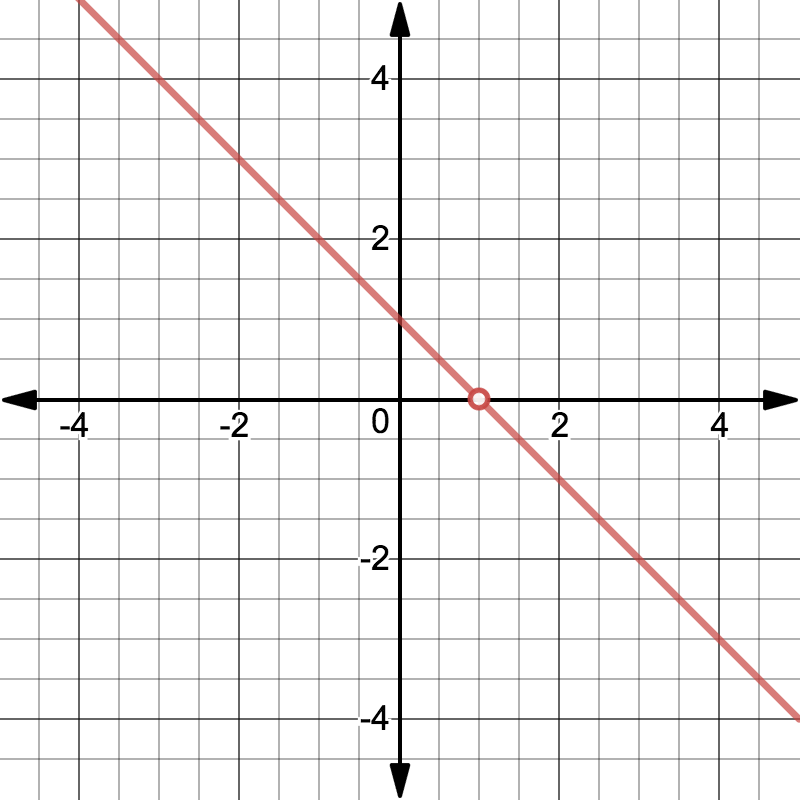
\includegraphics{continuity.png}
\end{image}

Through some simple elimination, we can easily see that this function is equivalent to $1-x$, where $x \neq 1$. Thus, there is one point on the original function we should pay close attention to: $x=1$.

Using the simple trick of squaring the denominator to create our numerator, we were able to easily pick a point where we will have a discontinuous function, without using a jump or infinite discontinuity. Jump discontinuities can easily be made using piecewise functions, and infinite discontinuities are often best made with rational functions, like fractions of polynomials! Don't worry if you haven't discussed these discontinuities yet; we'll see plenty in this lab!

\section{Problems}
\begin{question}
  Consider the graph of $y=f(x)$ below
  \begin{image}
    \begin{tikzpicture}
      \begin{axis}
    [xmin=-0.2,
          xmax=2.2,
          ymin=-0.2,
          ymax=2.2,
          axis lines=center,
          xlabel=$x$,ylabel=$y$,
          every axis y label/.style={at=(current axis.above origin),anchor=south},
          every axis x label/.style={at=(current axis.right of origin),anchor=west},
      domain=-1:2,
          clip=false,
      ytick={0.5,1,1.5,2},
      yticklabels={$0.5$,$1$,$1.5$,$2$},
      xtick={0.5,1.0,1.5,2},
      xticklabels={$0.5$,$1$,$1.5$,$2$},
      grid = major
    ]
        \addplot[very thick,black] plot coordinates {(0,0) (1,1)};
        \addplot[very thick,black] plot coordinates {(1,2) (2,0)};
        \addplot[color=black,fill=background,only marks,mark=*] coordinates{(1,1)};  %% open hole
        \addplot[color=black,fill=background,only marks,mark=*] coordinates{(.5,.5)};  %% open hole
         \addplot[color=black,fill=black,only marks,mark=*] coordinates{(0,0)};  %% closed hole
        \addplot[color=black,fill=black,only marks,mark=*] coordinates{(2,0)};  %% closed hole
        \addplot[color=black,fill=black,only marks,mark=*] coordinates{(1,2)};  %% closed hole

    \end{axis}
    \end{tikzpicture}
  \end{image}
  Which of the following are true?
  \begin{multipleChoice}
    \choice{$f$ is continuous at $x=0.5$}
    \choice{$f$ is continuous at $x=1$}
    \choice[correct]{$f$ is continuous at $x=1.5$}
  \end{multipleChoice}
\end{question}
\begin{question}
Create a function with the left handed and right handed limits not equal. What kind of discontinuity have you made here? Is there any kind of discontinuity that can't be created like this? Is there another that can?
Consider the function $$f(x) = \frac{x^3+6x^2+12x+8}{x+2} \text{,}$$ Describe the continuity of this function. If there is a discontinuity, where is it present? Is it possible to modify the function to remove this discontinuity? If so, how?
\begin{freeResponse}
\end{freeResponse}
\end{question}

\begin{question}
Consider the function $$g(x) = \frac{5x+2}{2x-3} \text{,}$$ Describe the continuity of this function. If there is a discontinuity, where is it present? Is it possible modify the function to remove this discontinuity? If so, how?
\begin{freeResponse}
\end{freeResponse}
\end{question}

\begin{question}
Design a function with a removable discontinuity at 2, and a jump discontinuity at 0.
\begin{freeResponse}
\end{freeResponse}
\end{question}

\begin{question}
Design a function with an infinite discontinuity and at least one other type of discontinuity
\begin{freeResponse}
\end{freeResponse}
\end{question}

\begin{dialogue}
\item[Julia] Whenever I see people talking about jump discontinuities, they always use piecewise functions. Do you think it's possible to make one without the function being piecewise?
\item[Dylan] If there's one thing that I've learned in math, it`s that there are usually two ways to do anything! I'm not really sure how you would make something like that though...
\item[James] I know one function that would work! Here's a hint - my function has one value on the positives, the opposite of that on the negatives, and is undefined at 0.
\end{dialogue}

\begin{question}
Can you create a function which has a jump discontinuity, but is \textit{not} piecewise?
\begin{freeResponse}
\end{freeResponse}
\end{question}

\begin{dialogue}
\item[Julia] Hey y'all, I was looking at our continuous graphs and noticed something.
\item[Dylan] What did you see? They all look like pretty normal functions to me.
\item[James] Yeah, I don't really know what you mean.
\item[Julia] Well, discontinuities mean there are a chunk of the graph where you can skip over a value, right? Like, we can jump right from 1 to 5, or have a hole where some value isn't attained.
\item[Dylan and James] Right. And?
\item[Julia] I think if we picked a continuous function and looked at the functional values on each end of a range, we could say something about all the values in between those two!
\end{dialogue}

\begin{question}
Can you create a function which has a jump discontinuity, but is \textit{not} piecewise?
\begin{freeResponse}
\end{freeResponse}
\end{question}

\begin{question}
\begin{hint}
Can we skip any of the values?
\end{hint}
What can we say about every value in a range $[f(a),f(b)]$ on a continuous graph?
\begin{freeResponse}
\end{freeResponse}
\end{question}



\end{document}

